\begin{frame}
\frametitle{Day 18: Lavaduct Lagoon}

    \begin{center}
        Given instructions consisting of direction and distance to dig out the edge of a pit, what will the resulting area of the pit be?
    \end{center}

\end{frame}

\begin{frame}[fragile]
\frametitle{Day 18: Example}
    
    \begin{center}
        \begin{minipage}{0.3\textwidth}
        \begin{center}
        \begin{verbatim}
R 6
D 5
L 2
D 2
R 2
D 2
L 5
U 2
L 1
U 2
R 2
U 3
L 2
U 2
        \end{verbatim}
        \end{center}
        \end{minipage}
        \begin{minipage}{0.3\textwidth}
        \begin{center}
        \begin{verbatim}
#######
#.....#
###...#
..#...#
..#...#
###.###
#...#..
##..###
.#....#
.######
        \end{verbatim}
        \end{center}
        \end{minipage}
        \begin{minipage}{0.3\textwidth}
            \begin{center}
            \begin{verbatim}
#######
#######
#######
..#####
..#####
#######
#####..
#######
.######
.######
            \end{verbatim}
            \end{center}
            \end{minipage}
    \end{center}
    \vfill

\end{frame}

\begin{frame}
\frametitle{Day 18: Bigmode}

Finding the area of these small shapes isn't too bad.\vfill

Could use a left-to-right scan, flood fill, whatever, and computationally be alright. But what if it was much bigger?\vfill

Part 2: Oops, instead of numbers from 2 to 12, we meant to give you a 5 digit hexadecimal number.\vfill

Our answer has now gone from a magnitude of 1e4 to 1e14.\vfill

\end{frame}

\begin{frame}
\frametitle{Day 18: Thinking with Shapes}

Storing and computing is now out of the question.*\vfill

New approach: thinking. What is it that we need the area of?\vfill

How can we get the area of that?\vfill

\end{frame}

\begin{frame}[fragile]
\frametitle{Day 18: Shoelace, Gauss, Surveyor's, etc.}

\begin{center}
$A = \frac{1}{2}\sum_{i=1}^{n}(y_i + y_{i+1})(x_i - x_{i+1})$\vfill
\end{center}

\begin{center}

\begin{minipage}{0.3\textwidth}
\begin{center}
\begin{verbatim}
A-----B
|.....|
N-M...|
..|...|
..|...|
K-L.D-C
|...|..
JI..E-F
.|....|
.H----G
\end{verbatim}
\end{center}
\end{minipage}
\begin{minipage}{0.3\textwidth}
\begin{center}
$(y_{A} + y_{B})(x_{A} - x_{B})$
$(y_{B} + y_{C})(x_{B} - x_{C})$
$(y_{C} + y_{D})(x_{C} - x_{D})$
$(y_{D} + y_{E})(x_{D} - x_{E})$
...
$(y_{N} + y_{A})(x_{N} - x_{A})$
\end{center}
\end{minipage}

\end{center}
\vfill

\end{frame}

\begin{frame}
\frametitle{Day 18: Pick's Theorem}

Our area calculation is still a smidge short.\vfill

If we consider ourselves to be digging out a cube block of dirt, we're standing in the center of the block and therefore not counting all of it when digging.\vfill

Enter Pick's Theorem: $A = i + \frac{b}{2} - 1$

\end{frame}

\begin{frame}
\frametitle{Day 18: Visualization}

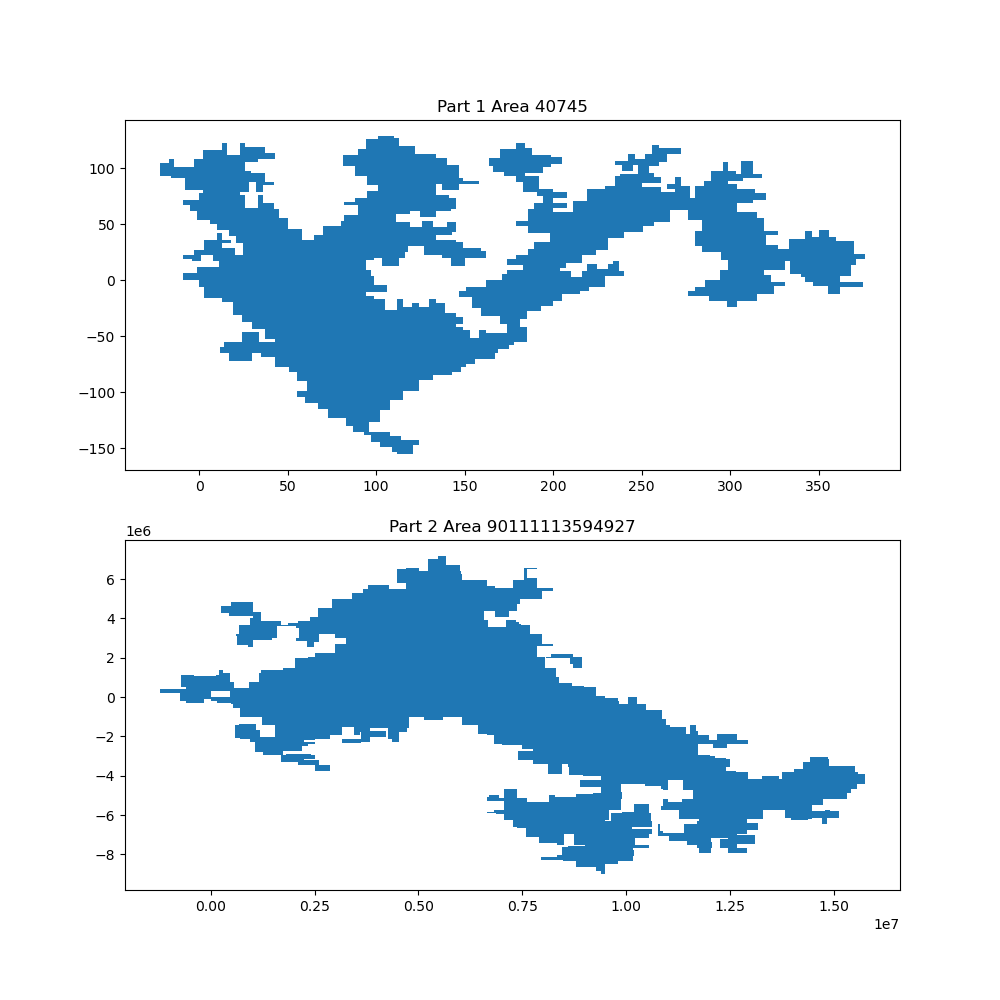
\includegraphics[height=\textheight]{Day18}

\end{frame}